% Figure source (ablations). Rendered to figures/pdf/ablations.pdf by the
% figure build; delete that PDF to have LaTeX compile this source instead.
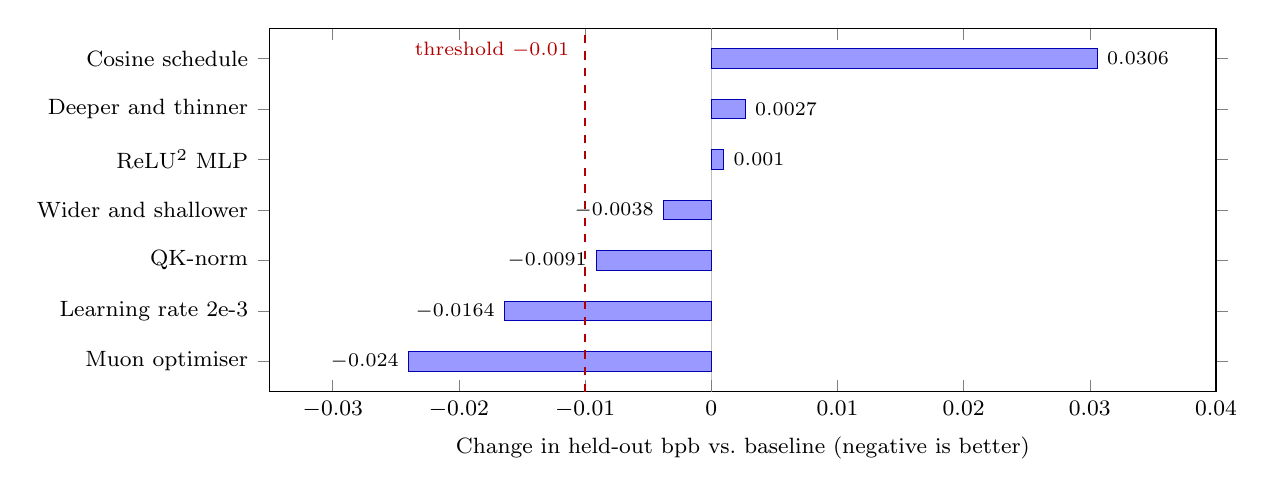
\begin{tikzpicture}
\begin{axis}[
    xbar, width=13.6cm, height=6.2cm,
    xlabel={Change in held-out bpb vs.\ baseline (negative is better)},
    symbolic y coords={cosine,deep,relu,wide,qknorm,lr,muon},
    ytick=data, y dir=reverse,
    yticklabels={Cosine schedule,Deeper and thinner,ReLU$^2$ MLP,Wider and shallower,QK-norm,Learning rate 2e-3,Muon optimiser},
    xmin=-0.035, xmax=0.04, bar width=7pt,
    nodes near coords, nodes near coords align={horizontal},
    every node near coord/.append style={font=\scriptsize, /pgf/number format/.cd, fixed, precision=4},
    tick label style={font=\footnotesize}, label style={font=\footnotesize},
    scaled x ticks=false,
    xticklabel style={/pgf/number format/.cd, fixed, precision=2},
    extra x ticks={0}, extra x tick style={grid=major, tick label style={opacity=0}}
]
\addplot[fill=blue!40, draw=blue!70!black] coordinates {
    (0.0306,cosine) (0.0027,deep) (0.0010,relu)
    (-0.0038,wide) (-0.0091,qknorm) (-0.0164,lr) (-0.0240,muon)};
\draw[red!70!black, dashed, thick] ({axis cs:-0.01,muon} |- {rel axis cs:0,0}) -- ({axis cs:-0.01,muon} |- {rel axis cs:0,1});
\node[font=\scriptsize, red!70!black, anchor=north east] at ({axis cs:-0.0105,muon} |- {rel axis cs:0,0.99}) {threshold $-0.01$};
\end{axis}
\end{tikzpicture}
